\documentclass[pdftex]{article}
% \documentclass[prl,showpacs,amsmath,amssymb]{revtex4} % PRL

% margins of 1 inch:
\setlength{\topmargin}{-.5in}
\setlength{\textheight}{9in}
\setlength{\oddsidemargin}{0in}
\setlength{\textwidth}{6.5in}

\usepackage[pdftex]{hyperref} % hyperlink equation and bibliographic citations
\usepackage[dvips]{graphicx,color}
\usepackage{amsmath} % advanced math
\usepackage{verbatim} % multi-line comments
\usepackage{natbib} % bibilography
\usepackage{mciteplus} % collapse multiple citations in bibilography

% from http://www.flakery.org/search/show/569

\newcommand{\infint}{\ensuremath{\int_{-\infty}^{\infty}}}

\newcommand{\ie}{\textit{i.e.}\ }
\newcommand{\eg}{\textit{e.g.}\ }

\newcommand{\eqn}[1]{Eq.\ (\ref{#1})}

\newcommand{\pfrac}[2]{\ensuremath{\frac{\partial #1}{\partial #2}}}

\begin{document}

\title{Network Model}

\author{Ben Payne$^{1}$\footnote{Electronic address: bpayne@lps.umd.edu}
{\it $^{1}$Department of Fun, University Name \& Town, city, State Zip}}

\date{\today}

% \begin{abstract}
% Model random networks
% \end{abstract}

%\maketitle % declares end of title page

%\tableofcontents

%\newpage

\section{Introduction}

There are two methods to model a network:
\begin{itemize}
 \item create a database of port connections
 \item create autonomous switches which direct packets to other components
\end{itemize}
For this model I will be using a database of connections.

\subsection{objectives}

If I can show a given topology is better than some other, that is useful.

If I can show how one switch versus another (differentiated by number of ports) affects performance, that is useful.

\subsection{Does Topology matter? A toy model example}

An optimal all-to-all design would have each compute node with $N-1$ ports and no switches (0 hops). For N>1000 this becomes difficult. Thus we introduce switches.

Suppose now we have $N=5$ compute nodes with 1 port each. Then the optimal network design (fewest hops) is to have a 5 port switch:

\begin{center}
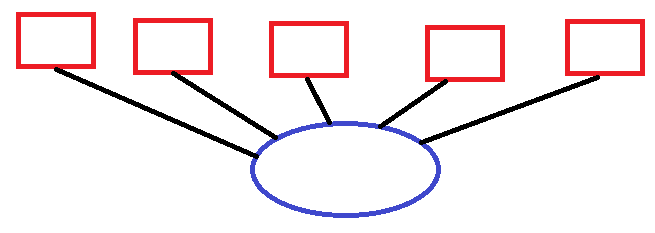
\includegraphics[scale=0.2]{S1_C5.png}\\*
\footnotesize{Here number of hops is 1 for each compute node, with 10 pairs (=5*4/2).}
\end{center}

The other extreme would be to use five of these same switches with only one compute node per switch:

\begin{center}
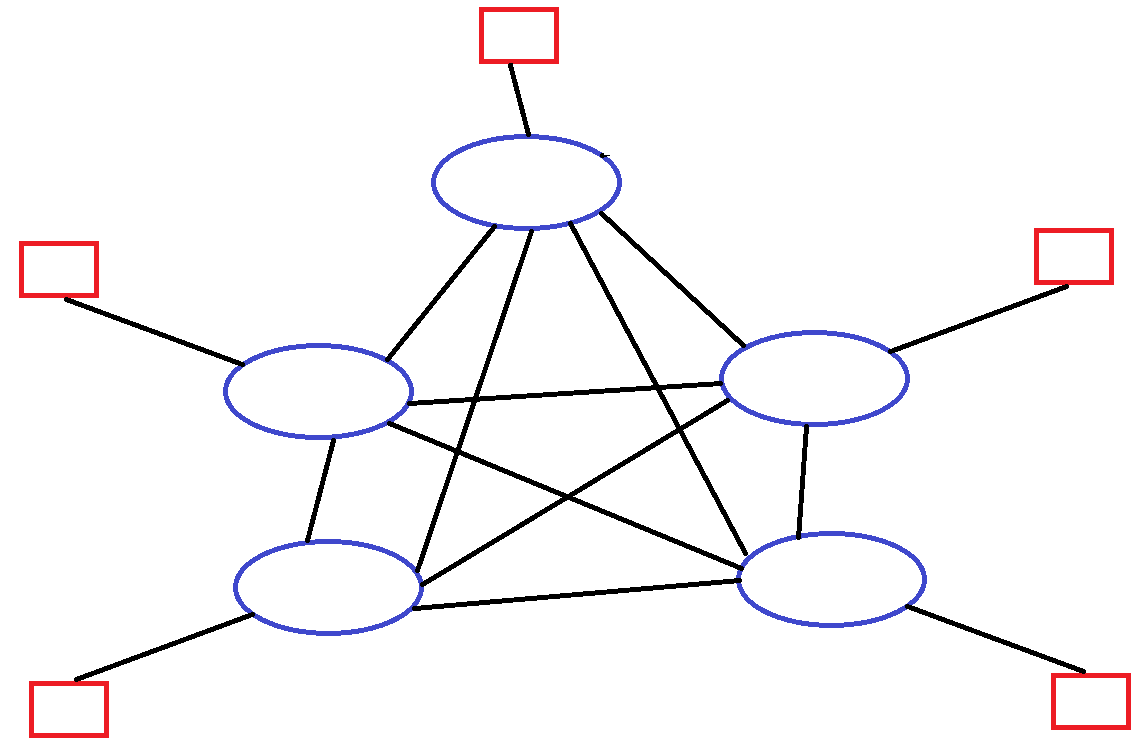
\includegraphics[scale=0.2]{S5_C5.png}\\*
\footnotesize{Here number of hops is 2 for each compute node.}
\end{center}
Clearly we are spending too much money on switches for the same number of compute nodes. However, this increased hop count (2) also lowers conjestion.

As a compromise, we can use two switches and increase the number of compute nodes:

\begin{center}
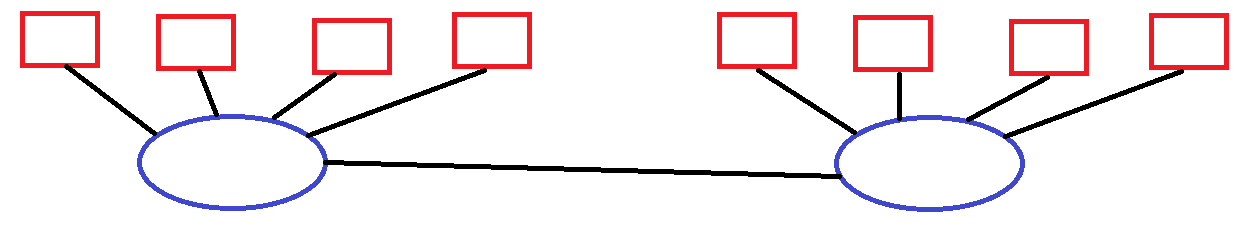
\includegraphics[scale=0.2]{S2_C8.png}\\*
\footnotesize{8 nodes and 2 switches: 12 pairs with 1 hop, 16 pairs with 2 hops.}
\end{center}

\begin{center}
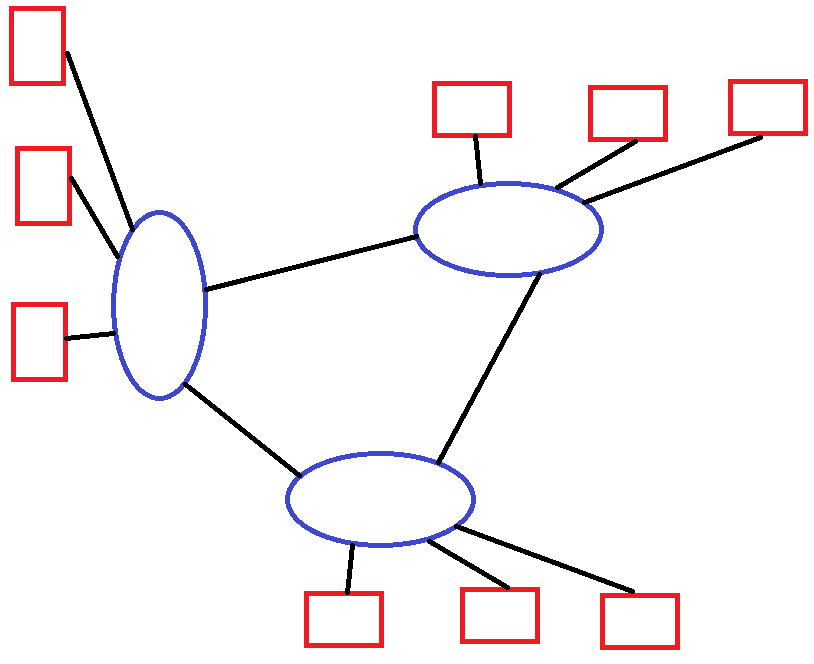
\includegraphics[scale=0.2]{S3_C9.png}\\*
\footnotesize{1 or 2 hops, 9 nodes and 3 switches.}
\end{center}

Notice a few constraints were followed:
\begin{itemize}
 \item each switch has same number of ports
 \item each compute node has one port
 \item each switch is fully occupied
 \item each node can reach every other node
 \item each switch has at least one computer connected to it
\end{itemize}

The number of permutations increases when we have more than 9 compute nodes and only 5 ports. Even worse, consider when there are multiple ports per computer (but much less than the number of computers).

The parameter space includes
\begin{itemize}
 \item number of computers
 \item number of ports per computer
 \item number of switches
 \item number of ports per switch
\end{itemize}
Metrics:
\begin{itemize}
 \item hop count for each pair
 \begin{itemize}
  \item average hop count
  \item maximum hop count
 \end{itemize}
 \item bisection bandwidth
\end{itemize}


\subsection{Permutations}

The number of unique pairs on a network swith $N$ computers is $N(N-1)/2$. 

When $N=4$ then there are 6 pairs. $N=100$ is 4950 pairs. $N=10,000$ is 49,995,000 pairs.

\section{standard networks}

See \href{http://www.cs.nmsu.edu/~pfeiffer/classes/573/notes/topology.html}{http://www.cs.nmsu.edu/~pfeiffer/classes/573/notes/topology.html}

\subsection{Mesh}
Mesh (and the related torus) can be of $n$ dimensions, commonly $n=$2, 3, 6. Useful for physical sciences due to local communication (nearest neighbors).
\begin{comment}
##Command to produce the output: "neato -Tpng thisfile.gv > thisfile.png"
##Command to produce the output: "circo -Tpng thisfile.gv > thisfile.png"
graph G {
node [shape=box,color=red,style=bold];  c0;
node [shape=box,color=red,style=bold];  c1;
node [shape=box,color=red,style=bold];  c2;
node [shape=box,color=red,style=bold];  c3;
node [shape=box,color=red,style=bold];  c4;
node [shape=box,color=red,style=bold];  c5;
node [shape=box,color=red,style=bold];  c6;
node [shape=box,color=red,style=bold];  c7;
node [shape=box,color=red,style=bold];  c8;
node [shape=circle,fixedsize=true,width=0.9,color=blue,style=bold];  s0;
node [shape=circle,fixedsize=true,width=0.9,color=blue,style=bold];  s1;
node [shape=circle,fixedsize=true,width=0.9,color=blue,style=bold];  s2;
node [shape=circle,fixedsize=true,width=0.9,color=blue,style=bold];  s3;
node [shape=circle,fixedsize=true,width=0.9,color=blue,style=bold];  s4;
node [shape=circle,fixedsize=true,width=0.9,color=blue,style=bold];  s5;
node [shape=circle,fixedsize=true,width=0.9,color=blue,style=bold];  s6;
node [shape=circle,fixedsize=true,width=0.9,color=blue,style=bold];  s7;
node [shape=circle,fixedsize=true,width=0.9,color=blue,style=bold];  s8;
     s0--c0;
     s1--c1;
     s2--c2;
     s3--c3;
     s4--c4;
     s5--c5;
     s6--c6;
     s7--c7;
     s8--c8;
     s0--s1; 
     s0--s3;
     s1--s2;
     s1--s4;
     s2--s5;
     s3--s4;
     s3--s6;
     s4--s7;
     s4--s5;
     s5--s8;
     s6--s7;
     s7--s8;
     overlap=false
     label="3x3 mesh\nlayed out by Graphviz"
     fontsize=12;
}
\end{comment}
Mesh networks are well-characterized. ``Meshes have O(n) cost, O(sqrt(n)) bisection bandwidth, O(n) aggregate bandwidth, and O(sqrt(n)) latency.''

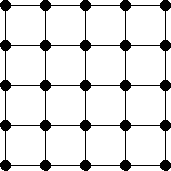
\includegraphics[scale=.5]{mesh.png}

\subsection{Hypercube}

``the latency is is O(log N). There are N processors, each with log2N interfaces, so the cost is O(N log N). and all the processors can use their links simultaneously, so our aggregate bandwidth is O(N). The bisection bandwidth is O(log N).''

\subsection{Fat Tree}

\href{http://en.wikipedia.org/wiki/Fat_tree}{http://en.wikipedia.org/wiki/Fat\_tree}

\subsection{Flattened Butterfly}

\subsection{Dragonfly}

\href{http://research.google.com/pubs/pub34926.html}{http://research.google.com/pubs/pub34926.html}

Fractal

\subsection{Clos Network}

\href{http://en.wikipedia.org/wiki/Clos_network}{http://en.wikipedia.org/wiki/Clos\_network}

\subsection{randomly-connected networks}

For networks supporting physical models (i.e., mesh), it makes sense to think about dimension, perimeter/surface area, area/volume. This may not apply to scale-free topologies. 

If the topology turns out to be scale free, then we wouldn't need to model 1E6 endpoints (that is desirable).

\section{more than one port per endpoint}

If each endpoint has only one network connection, then we can model a switch-only network. A switch with 4 ports not connected to other switches would have 4 endpoints.

\section{random network creation}

For a given \{(number of computers), (number of ports per computer), (number of ports per switch)\}, should random computers be plugged into random port switches, or should random switches be connected first?

\ \\
``connections'' database methods:
\begin{itemize}
 \item each switch is an sub-array of the connections array. The elements of each sub-array denote which computer the switch is plugged into. 
 \item connections pairs: computer--switch and switch-switch. The connections array has sub-arrays of size 2 for each edge of the graph (nodes are either computers or switches).
 \begin{itemize}
  \item unordered pairs of positive (switch) and negative (computer) integer indices
 \end{itemize}

\end{itemize}
Features needed:
 \begin{itemize}
  \item supports switches having arbitrary port count (not all switches must have same number of ports
 \end{itemize}


\ \\
Whether local symmetry (same number of computers plugged into each switch) is a hinderance, benefit, or irrelevant is not clear to me.

Random connections lead to unexpected paths. This could be good, bad, or inconsequential.

\section{route enumeration}

\begin{enumerate}
 \item For each computer, see what other computers are available on the same switch (1 hop)
 \item For each computer, see what other computers are two switches away (2 hops)
 \item ...
\end{enumerate}
When a switch has had all of its computers touched for a given iteration, then we should mark that switch as ``touched'' (doesn't need to be queried again for current iteration). That is, mark a switch to indicate ``all locally-attached computers have number of hops known.'' This should reduce search time.

\section{future task list}

Once the hop counter is implemented, it would be useful to validate it against analytic values for mesh, torus, fat tree topologies.


\end{document}
